\chapter{Scientific Programming}

The introduction of the computer around 1945 had a major impact on the mathematical fields of science. Previously unsolvable problems were now easily solvable. The question was no longer whether or not it was possible, but rather to what precision and with which method. The computer spawned a new branch of physics, \textit{computational physics}, breaching barriers no one could even imagine existed. The first major result of this synergy between science and computers came with the atomic bombs as a result of the Manhattan Project at the end of the second world war \textbf{citation needed}.       

\section{Programming languages}

Writing a program, or a code, is a list of instructions for the computer. It is in many ways similar to writing human-to-human instructions. You may use different programming languages, such as C++, Python, Java, as long as the reader is able to translate it. The translator, called \textit{compiler}, translates your program from e.g. C++ code into machine code. Other languages as Python are interpreted real-time and therefore require no compilation. Although the latter seems like a better solution, it comes at the price of efficiency, a key concept in programming. 

As a rule of thumb, efficiency is inverse proportional to the complexity of the programming language. It is therefore natural to sort languages into different subgroups depending on where they are at the efficiency-complexity scale.


\subsection{High-level languages}

This subgroup of languages are often referred to as \textit{scripting languages}. A script is a short code, often with a specific purpose such as analyzing output by e.g. generating tables and figures from raw data, or gluing together different programs which are meant to be run in sequential order.

For simple jobs as these, taking only seconds to run on modern computers, we do not need an optimized code, but rather an easily read, clutter-free code. The languages which prefer simplicity over efficiency are referred to as \textit{High-level} \footnote{There are different definitions of high-level vs. low-level. You have languages such as \textit{assembly}, which is extremely complex and close to machine code, leaving all machine-independent languages as high-level ones. However, for the purpose of this thesis I will not go into assembly languages, and keep the distinction at a higher level.}. Examples of high-level languages are Python, Ruby, Perl, Visual Basic and UNIX shells. In this thesis I will emphasize the use of Python as a scripting language.   

\subsubsection{Python}
\label{sec:Python}

Python is an open source programming language with a focus on simplicity over complexity. To mention a few of the entries in the \textit{Zen of Python}\footnote{Retrieved by typing ``import this'' in your Python shell.}, ``Beautiful is better than ugly. Simple is better than complex. Readability counts. If the implementation is hard to explain, it's a bad idea.''

To demonstrate the simplicity of Python, let us have a look at a simple implementation and execution of the following expression

\[
 S = \sum_{i=1}^{100} i = 5050.  \label{eq:sum100}
\]

\lstinputlisting[language=Python]{../CodeInputs/Sum100Python.py}


\begin{verbatim}
~$ python Sum100Python.py 
5050
\end{verbatim}




\subsection{Low-level languages}
\label{sec:lowlevel}

A huge part of scientific programming is solving complex equations. Complexity does not necessarily imply that the equations themselves are hard to understand. Frankly, this is often not the case. In most cases of linear algebra, the problem can be boiled down to solving $A\vec x = B$, however, the complexity lies in the dimensionality of the problem at hand. Matrix dimensions range as high as millions. With each element being a double precision number, it is crucial that we have full control of the memory, and execute operations as efficiently as possible. 

This is where lower level languages excel. Hiding few to none of the details, the power is in the hand of the programmer. This comes at a price. More technical concepts such as memory pointers, declarations etc. makes the development process slower than that of a higher-level language. If you e.g. try to access an element outside the bounds of an array, Python would tell you exactly this, whereas C++ would crash runtime leaving nothing but a ``segmentation fault'' for the user to interpret. However, when the optimized program ends up running for days, the extra time spent developing it pays off. As a rule of thumb, higher-level languages (without focus on \textit{vectorization} or other optimization techniques) run 100 times slower than lower level ones. 

\subsubsection{C++}

C++ is a language developed by Bjarne Stroustrup in 1979 at Bell Labs. It serves as an extension to the original \textit{C} language, adding e.g. object oriented features such as classes. To calculate the sum in Eq.~\ref{eq:sum100} with C++, we would need something like this:

\vspace{0.5 cm}
\lstinputlisting[language=c++]{../CodeInputs/Sum100C++.cpp}

\begin{verbatim}
~$ g++ Sum100C++.cpp -o sum100C++.x
~$ ./sum100C++.x 
5050
\end{verbatim}


As we can see in lines five and six, we need to declare \textit{S} and \textit{i} as integer variables, exactly as described in section~\ref{sec:lowlevel}. In comparison with the Python version, it is clear that lower level languages are more complicated, and not designed for simple jobs as calculating a single sum.

Even though this is an extremely simply example, it illustrates the difference in coding styles between high- and low-level languages: Complexity vs. simplicity, efficiency vs. readability. I will not go through all the basic details of C++, but rather focus on the more complicated parts involving object orientation in scientific programming.


\section{Object orientation}
\label{sec:OO}

Object orientated programming was introduced in the language \textit{Simula}, developed by the Norwegian scientists Ole-Johan Dahl and Kristen Nygaard\textbf{Need specifics and citations}. It quickly became the state-of-the-art in programming, and is today used throughout the world in all branches of programming. It is brilliant in the way that it ties our everyday intuition into the programming language - our brain is object oriented. It is focused around the concept of \textit{classes}, an extension to standard \textit{structs}. A class is nothing but a collection of variables and functions under a sensible name, however, they provide a great deal of functionality like \textit{inheritance} and accessibility control. To better illustrate the concept of classes and inheritance, let us first look at an example.

\subsection{Inheritance}

All keyboards have two things in common: A board and keys. In object orientation we would say that the \textit{superclass} of keyboards describe a board with keys. It is \textit{abstract} in the sense that you do not need to know what the keys look like, or what function they possess, in order to define the concept of a keyboard.

However, we can have different types of keyboards, for example a computer keyboard, or a musical keyboard. They are different in design and function, but they both relate to the same concept of a keyboard described previously. They are both \textit{subclasses} of the same superclass, inheriting the basic concepts, but expands upon them defining their own specific case. Let us look at how this concept can be converted into Python code

\vspace{0.5 cm}
\lstinputlisting[language=Python]{../CodeInputs/KeyboardClassPython.py}

As we can see, the only thing differentiating the two keyboard types are how the keys are set up, and what happens when we press one of them. A superclass function designed to be overridden is referred to as \textit{virtual}. 

\subsection{Virtual Functions, pointers and types}

It a virtual function is overridden, the latest implementation will be called. \verb+setupKeys+ and \verb+pressKey+ are examples of this, however, they are in a sense more than virtual, since they are not even implemented. They have to be overridden in order to work. These functions are referred to as \textit{pure virtual} functions. In python, all class functions, or member functions, are virtual. In C++ however, we have to specify whether or not a function is virtual in the declaration. 

Higher level languages like Python handles all the pointers by itself. In low-level languages like C++, however, you need to control these yourself. A pointer is a hexadecimal number representing a memory address. If you pass a pointer to an object, e.g. \verb+Someclass* someobject+, as an argument to a function, whenever that function changes a class variable, the value is changed globally, since the memory address is directly accessed. If you instead choose to send the object without a pointer declaration, e.g. \verb+Someclass someobject+, changing the value will not change the object globally. What happens instead is that you change a local copy of the object. It is a misconception that pointers are your enemies, they are, quite frankly, making your codes much easier.

A pointer holds a type, that is, \verb+int+, \verb+double+, or any class that you have access to. In the following example we will study the interplay between virtual functions, pointers and types:

\vspace{0.5 cm}
\lstinputlisting[language=c++]{../CodeInputs/virtualFunctionsC++.cpp}

\begin{verbatim}
~$ ./virtualFunctionsC++.x 
-Calling subclass object of type VirtualTest*
subclass virtualFunc called
superclass notVirtualFunc called

-Calling subclass object of type subclass*
subclass virtualFunc called
superclass notVirtualFunc called

-Directly calling object of type subclass*
subclass virtualFunc called
subclass notVirtualFunc called
\end{verbatim}

In the first call, the pointer is declared as a \verb+VirtualTest*+ type, however, it is still initialized to be a subclass pointer in the sense that the subclass' functions are loaded into the object. This results in the virtual function being overridden (as mentioned previously), but since the object type is \verb+VirtualTest*+, C++ does not dig deeper than the superclass when it looks for the non-virtual function implementation. In other words: \verb+virtual+ induce a search for deeper implementations of the same function, given that the function is loaded through e.g. \verb+new subclass()+. 

In the second call, the same thing happens, even though it is set as a \verb+subclass*+ type. This is because the function is instructed to receive a superclass object. If it receives anything else, it simply attempts to convert it, or \textit{cast} it to a different type; \textit{typecasting}\footnote{The standard example of typecasting is converting a double to an integer, resulting in the stripping of all the decimal bits (flooring).}. In this case it works just fine. The third call, outside the function, demonstrates that if we declare it as a subclass type, both functions are overridden, since we do not have to go through the superclass at all.

The strength of using virtual functions in a class hierarchy is that you can easily expand or implement new functionality without completely rewriting the code. As an example, in the \verb+QMC+ code, changing potentials, or switching between closed form and numerical expressions for the dell and laplacian, is just a matter of which object's functions are called by the energy function.

\vspace{0.5 cm}
\begin{lstlisting}
double QMC::calculate_local_energy(Walker* walker) const {
    return kinetics->get_KE(walker) + system->get_potential_energy(walker);
}
\end{lstlisting}

\begin{lstlisting}
class Walker {
...

    mat r;
...
};
\end{lstlisting}

\begin{lstlisting}
class Kinetics {
...

    virtual double get_KE(const Walker* walker) = 0;
...
};

class Numerical : public Kinetics {
...

    virtual double get_KE(const Walker* walker);
...
};
\end{lstlisting}

\begin{lstlisting}
class Potential {
...

    virtual double get_pot_E(const Walker* walker) const = 0;
...
};

class Harmonic_osc : public Potential {
...
   
   virtual double get_pot_E(const Walker* walker) const;
...
};
\end{lstlisting}

\begin{lstlisting}
double Harmonic_osc::get_pot_E(const Walker* walker) const {

    double e_potential = 0;

    for (int i = 0; i < n_p; i++) {
        e_potential += 0.5 * w * w * walker->get_r_i2(i);
    }

    return e_potential;
}
\end{lstlisting}





The \verb+QMC+ member function receives a \verb+Walker*+ object, representing a set of positions for all particles. The \verb+kinetics+ object is of type \verb+Kinetics*+ and holds implementations of either a numerical calculation or a method for extracting closed form expressions from the orbitals. The \verb+get_potential_energy+ method is not virtual. It's purpose is to iterate over all potentials given (i.e. a Harmonic Oscillator and Coulomb), extracting their value at the walker's position. Adding a new potential to this list is extremely simple. 

The point is that the local energy function is written completely independent of how the potential actually looks. The implementation of a new potential would mean a new subclass of \verb+Potential+ with a new implementation of the virtual function \verb+get_local_E+. This makes the code extremely readable (given it is properly commented), since the reader would not have to care about the details if the algorithm is that of interest (and vice versa).

\subsection{Const Correctness}

In the \verb+QMC+ code example above, function declarations with \verb+const+ are used. If an object is declared with \verb+const+ on input, e.g. \verb+void f(const x)+, the function itself cannot alter the value of \verb+x+. It is a safeguard that nothing will happen to \verb+x+ as it passes through \verb+f+. This is practical in situations where major bugs will arise if anything happens to an object.

If you declare a member function itself with \verb+const+ on the right hand side, it safeguards the function from changing any of the class variables. If you e.g. have a variable representing the electron charge, you do not want this changed by the Coulomb class member function. This should only happen through specific functions whose sole purpose is changing the charge, and taking care of any following consequences. 

In other words: \verb+const+ works as a safeguard for changing values which should remain unchanged. A change in such a variable is then followed by a compiler error instead of infecting your code with bugs, resulting in unforeseen consequences.

\subsection{Accessibility levels and Friend classes}

\verb+const+ is a direct way to avoid any change what so ever. However, sometimes we want to keep the ability to alter variables, but only in certain situations, as e.g. internally in the class. As an example, from the main file, you should not have access to \verb+QMC+ member functions such as \verb+dump_output+, since it does not make sense to do out of a context. However, you obviously want access to the \verb+run_method+ function.

The solution to this problem is to set accessibility levels. Declaring a variable under the \verb+public+ part of a class sets its accessibility level to \textit{public}, meaning that anything, anywhere can access it as long as it has access to the object. All public variables are inherited to subclasses when inherited as in the virtual function example\footnote{You could inherit with protected option as well, but it is rarely used and messes up the functionality.}. Declarations beneath the \verb+private+ part stops all other classes than instances of it self from reaching it, even subclass instances. If you want private variables inherited, the \verb+protected+ accessibility level should be used.

There is one exception to the rule of protected and private variables, namely \textit{friend} classes. In the \verb+QMC+ library, there is a output class called \verb+OutputHandler+. This class needs access to protected variables, since the user should be able to output anything he wants. If we \verb+friend+ the output class with \verb+QMC+, we get exactly this behavior: 

\vspace{0.5 cm}
\begin{lstlisting}[language=c++]
class QMC {
protected:

    int n_c;

    int n_p;
    int n2;
    int dim;

    int cycle;

    ...
    
    Walker* original_walker;
    Walker* trial_walker;

    ...
    
public:
...

    friend class Distribution;
...
};
\end{lstlisting}

\begin{lstlisting}[language=c++]
void Distribution::dump() {

    if ((qmc->cycle > qmc->n_c / 2) && (qmc->cycle % 100 == 0)) {
        for (int i = 0; i < qmc->n_p; i++) {
            for (int j = 0; j < qmc->dim; j++) {
                if (j == qmc->dim - 1) {
                    file << qmc->original_walker->r(i, j);
                } else {
                    file << qmc->original_walker->r(i, j) << " ";
                }
            }
            file << endl;
        }
    }

}
\end{lstlisting}

Without going into details, we can see that \verb+Distribution+ has full access to protected members of \verb+QMC* qmc+. Friend classes is a savior in those very specific cases when you really need full access to protected members of another class, but setting full public access would ruin the code. It is true that you could code your entire code without \verb+const+ and with solely public members, but in that case, it is very easy to put together a very disorganized code, with pointers flying everywhere and functions being called in all sorts of contexts. Clever use of accessibility levels will make your code easier to develop in an organized, intuitive way - you will be forced to implement things in an organized fashion.


\subsection{Example: PotionGame}
\label{sec:PotionGame}

To end the section I would like to demonstrate the versatile power of object orientation. Consider the following codes (libraries)

\vspace{0.5 cm}
\lstinputlisting[language=Python]{../CodeInputs/potionClass.py}
\lstinputlisting[language=Python]{../CodeInputs/playerClass.py}

We have a \verb+Player+ class keeping track of a players energy and health level, and which potions the player is carrying. The \verb+Potion+ class described all potions, that is, an object of type \verb+Potion+ with the ability to affect a player in some way. The subclasses define specifically which effect is to be applied, e.g. \verb+HealthPotion+ changes the health level of the player by a certain amount. This code does nothing by itself, but let us use it in an example where two players fight each other:

\vspace{0.5 cm}
\lstinputlisting[language=Python]{../CodeInputs/potionGameMain.py}

\begin{verbatim}
~$ python potionGameMain.py 

Round start: 
john (hp/e=100/100):
Health Potion (10)
Energy Potion (30)

james (hp/e=100/100):
Energy Potion (20)
Energy Potion (20)


Player2 hit Player1 for 50 using 100 energy
Players used all potions
Player1 hit Player2 for 40 using 90 energy


Round 1: 
john (hp/e=60/10):
No potions aviable

james (hp/e=60/40):
No potions aviable

\end{verbatim}


The readability of this code is pretty good. Imagine if we had no objects, but just a lot of parameters per player juggled around in variables such as \verb+Player1health+ etc. Increasing the number of players then requires a total rewriting of the entire program, where as in this object oriented style, it is just a matter of adding another player object. Object orientation is truly brilliant when it comes to developing codes. 

In this section I have not focused too much on scientific computing, but rather on the use of object orientation in general. When the physical methods are discussed in section \textbf{Insert physics section}, I will get back to a more specific description of scientific programming.

As an introduction to the next section, take a look at the way the classes and the main file are separated in this section's example. In a small code like this there's really no point of doing so, but when the class structures span thousands of lines, having a good structure and the right editor is crucial to the development process and the code's readability.


\section{Structuring the code}

Structuring a code is another source of compromises. If the code is short, and has a direct purpose, e.g. to calculate the sum from Eq.~(\ref{eq:sum100}), structure is not an issue at all, given that reasonable variable names are provided. However, if the code is more complex, and the methods used are specific implementations of a more general case, e.g. integration, code structuring becomes very important. For details about the structuring of the code used in this thesis, see Section~\ref{sec:StructureandImplementation}.

The case of using object orientation with focus on code structure is covered in Section~\ref{sec:OO}.

\subsection{File structures}

If a code consists of several independent class structures, it is common to gather the data from the different classes in separate files (see Section~\ref{sec:PotionGame} for an example). The alternative would be a single file consisting of thousands of lines; navigating through it is a mess. This would not be so bad if the process of writing the code was linear, however, empirical evidence suggests otherwise; at least half the time is spent debugging functions.

All source code files should be gathered in a \textit{src} folder, with one folder per new class. Subclasses should appear as folders inside the superclass folders. 

\begin{figure}
 \label{FIG:SRCdirTree}
 \begin{center}
  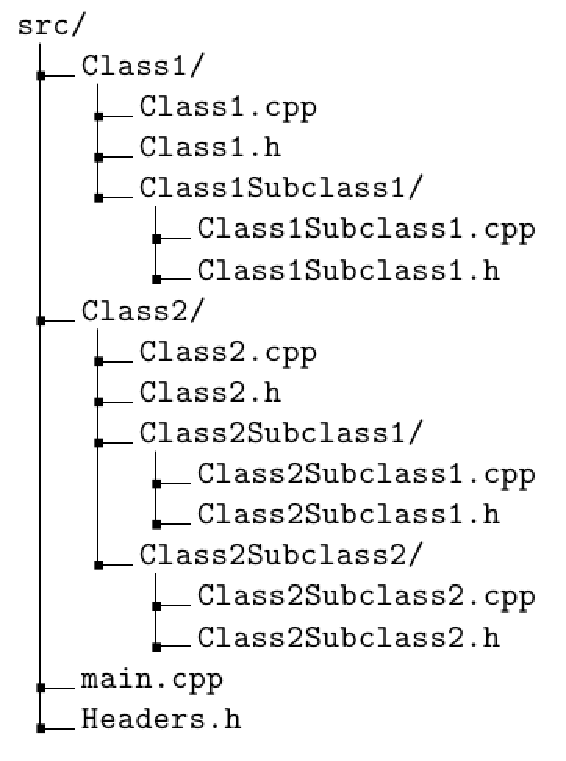
\includegraphics[scale=0.6]{../Graphics/SRCfolderStruct.pdf} 
 \end{center}
 \caption{An illustration of a standard way to organize source code. The file endings represent C++ code.}
\end{figure}


\subsection{Optimization and Profiling}

\subsection{IDEs}

Netbeans good yes, spider good yes